%\documentclass[main]{subfiles}

%\begin{document}

\vspace{-5pt}
\section{Experiments}
\label{sec:experiments}
\vspace{-3pt}


We evaluate EigenVI on 9 synthetic targets and 8 real data targets.
In these experiments we use the orthogonal family induced by
\emph{normalized Hermite polynomials} (see \Cref{tab:onedim}),
whose lowest-order expansion is  Gaussian.
Thus, this variational family can model non-Gaussian behavior with the higher-order functions in its basis.
We first study 2D synthetic targets and use them to demonstrate the expressiveness of
these higher-order expansions.
Next, we experiment with target distributions where we systematically vary the tail heaviness and amount of skew.
Finally, we apply EigenVI to a set of hierarchical Bayesian models from real-world
applications and benchmark its performance against other Gaussian BBVI algorithms.

\subsection{2D synthetic targets}

We first demonstrate how higher-order expansions of the variational family
yield more accurate approximations on a range of 2D non-Gaussian target distributions
(\Cref{fig:2dtargets});
see \Cref{ssec-2dsynthetic} for details.
We report an estimate of $\KL(p;q)$ above each variational approximation.
The Gaussian variational approximation is fit using batch and match VI~\citep{cai2024},
which minimizes a score-based divergence.
For EigenVI,
the target distributions were not standardized before fitting EigenVI
(we compare the costs of the methods in \Cref{fig:2dtargets-metrics}),
and the total number of basis functions is $K\!=\!K_1 K_2$.
%

\begin{figure*}[t]
    \centering
    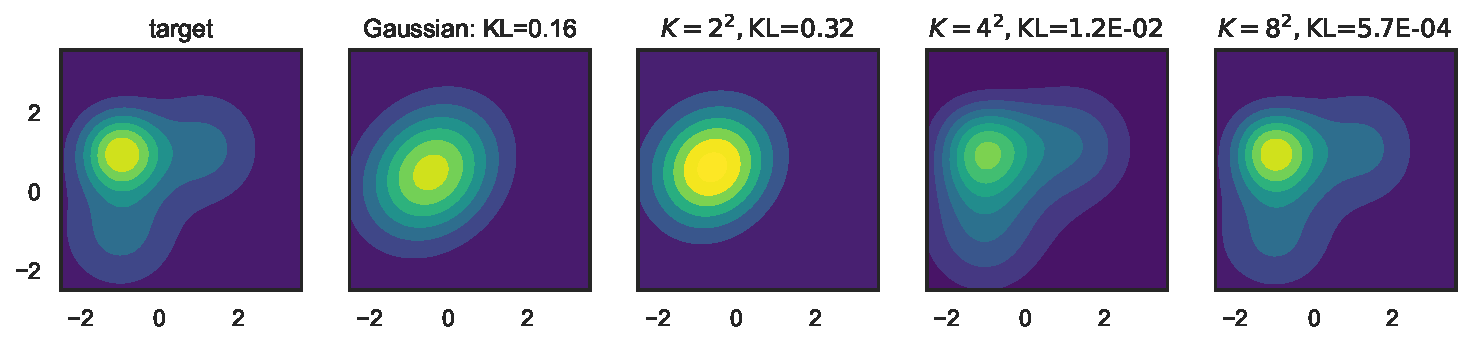
\includegraphics[scale=0.44]{figs/expts-2d-new/density-3gmm-full.pdf}
    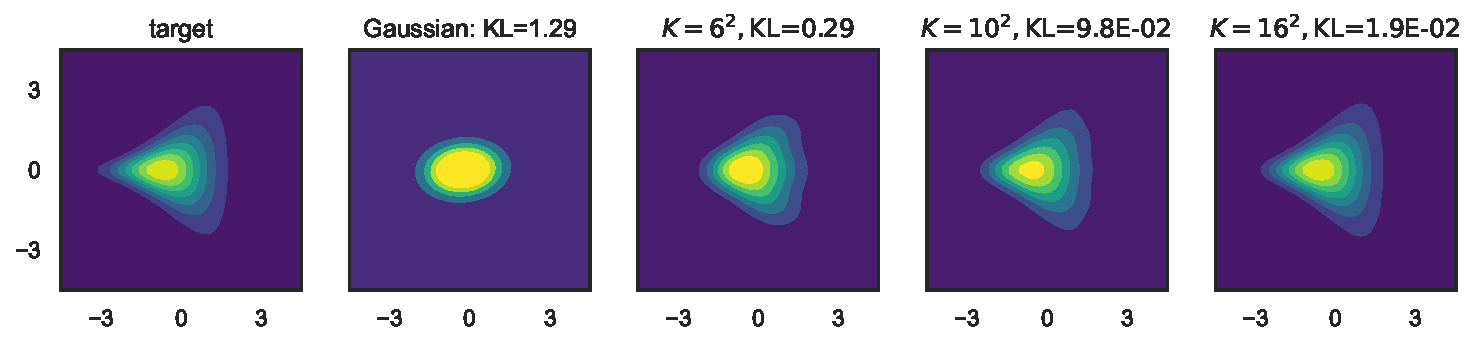
\includegraphics[scale=0.44]{figs/expts-2d-new/density-funnel-full.pdf}
    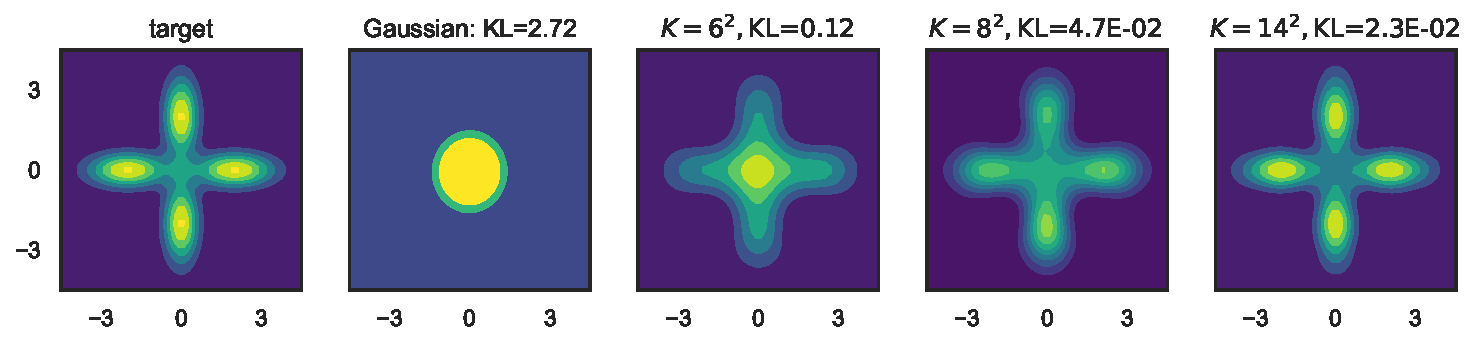
\includegraphics[scale=0.44]{figs/expts-2d-new/density-cross-full.pdf}
\caption{2D target functions (column 1): a 3-component Gaussian mixture distribution (row 1), a
funnel distribution (row 2), and a cross distribution (row 3).
    We report the $\KL(p;q)$ for the resulting optimal variational distributions obtained
    using score-based VI with a Gaussian variational family (column 2)
    and the EigenVI variational family (columns 3--5),
    where $K\!=\!K_1K_2$.
    }
\vspace{-10pt}
\label{fig:2dtargets}
\end{figure*}



\subsection{Non-Gaussianity:\ varying skew and tails in the sinh-arcsinh distribution}

\begin{figure*}[t]
    \centering
    \begin{subfigure}[b]{\linewidth}
    \centering
    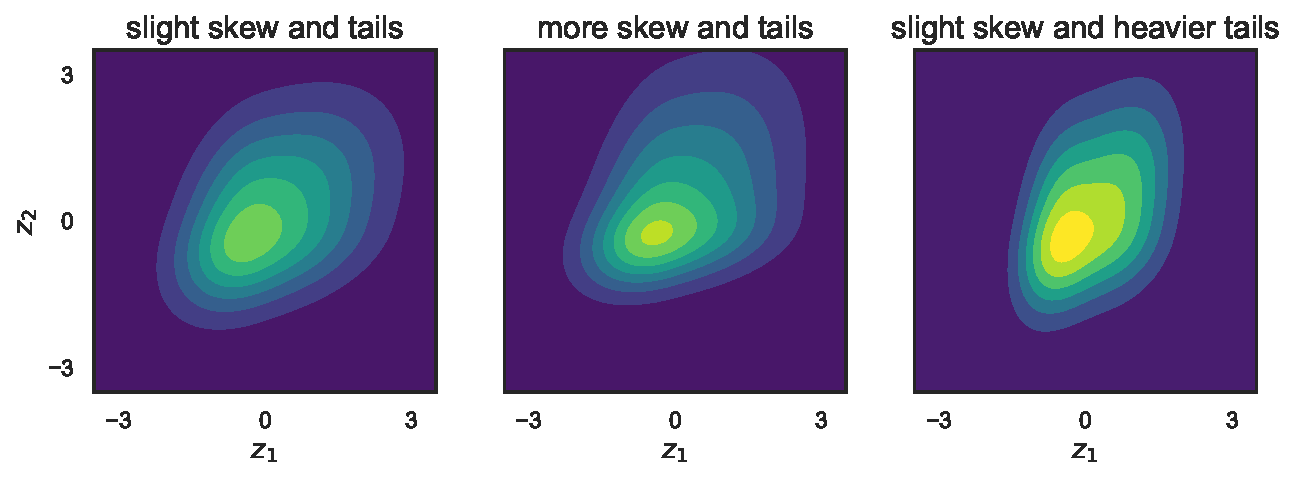
\includegraphics[scale=0.32]{figs/expts-2d-new/sinh-varied2.pdf}
    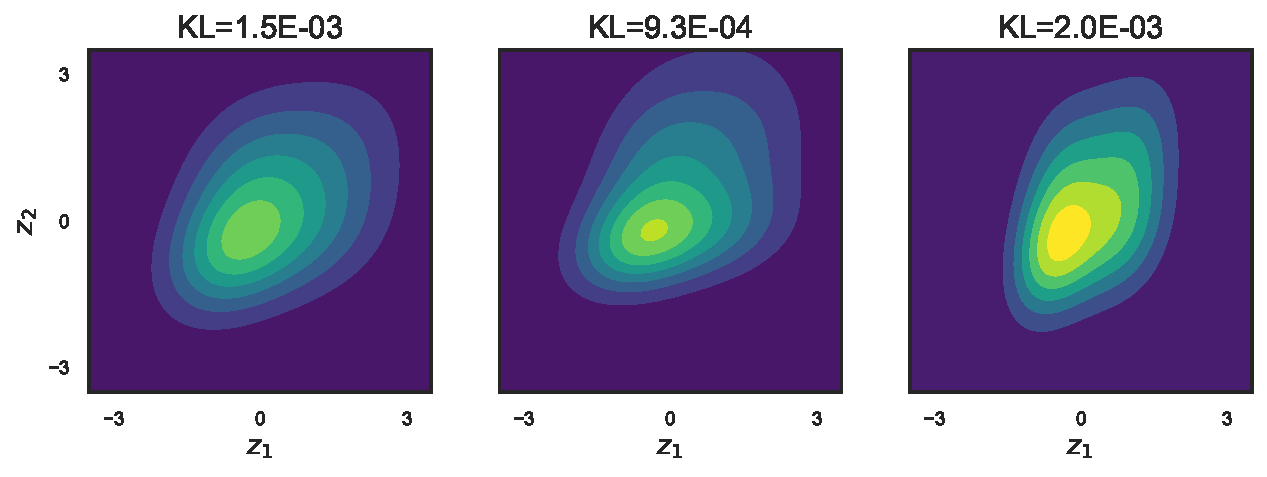
\includegraphics[scale=0.32]{figs/expts-2d-new/sinh-varied2-fits.pdf}
    \caption{Example 2D targets (left)  varying the skew $s$ or tail weight $\tau$
    components and their EigenVI fits (right).
    }
    \label{fig:sinh2dtargets}
\hspace{10pt}
    \end{subfigure}
    \begin{subfigure}[b]{\linewidth}
        \centering
    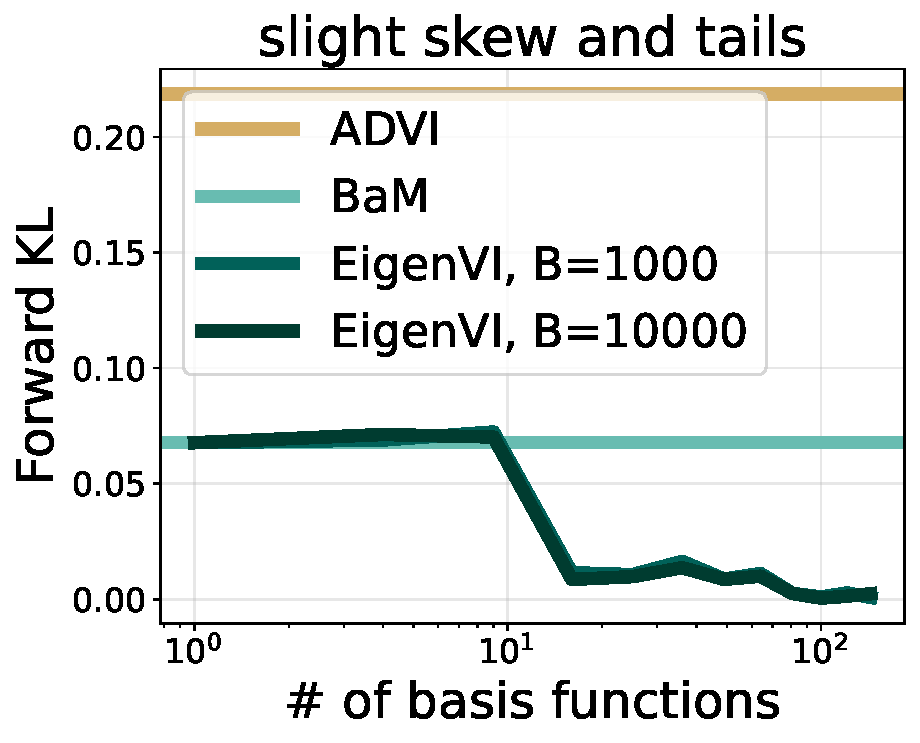
\includegraphics[scale=0.21]{figs/expts-2d/sinh-2D-P1-new.pdf}
    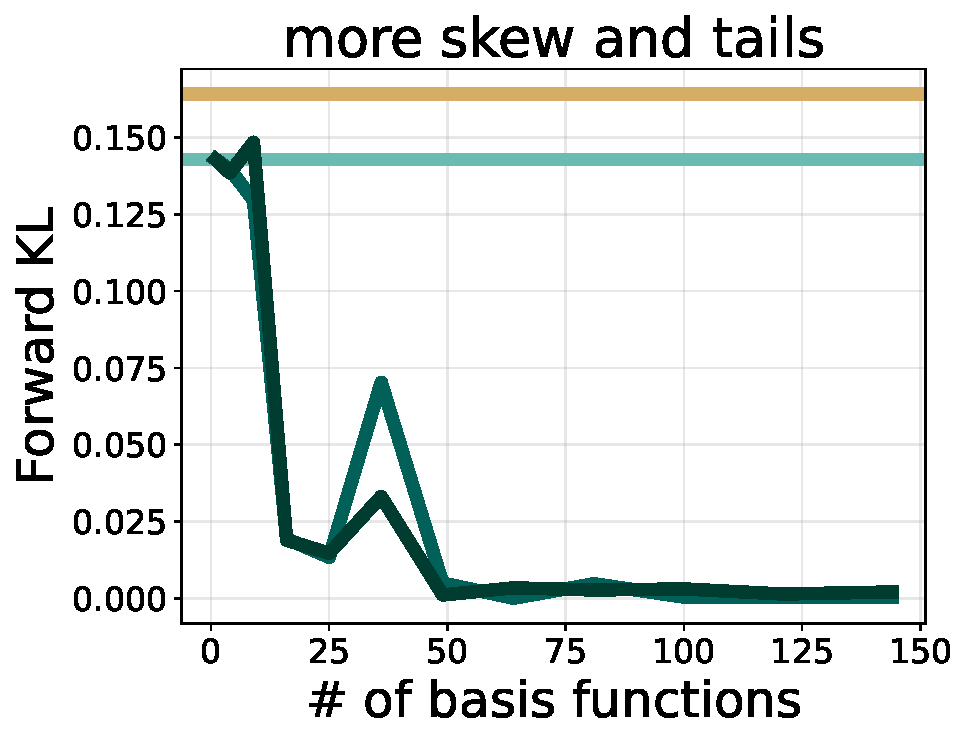
\includegraphics[scale=0.21]{figs/expts-2d/sinh-2D-P2-new.pdf}
    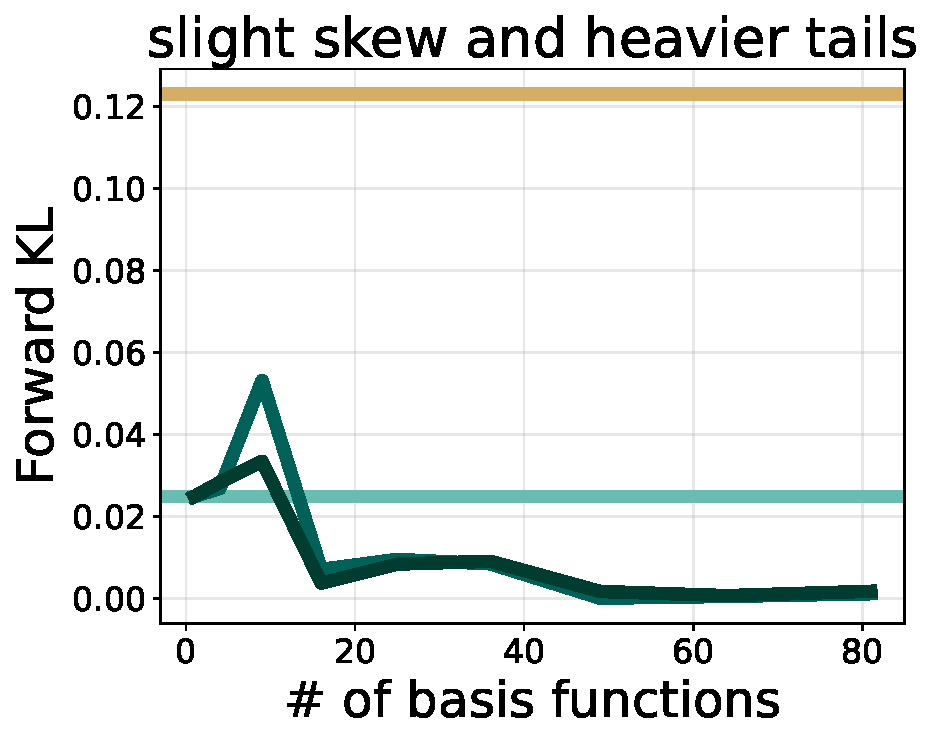
\includegraphics[scale=0.21]{figs/expts-2d/sinh-2D-P3-new.pdf}
\caption{$D=2$}
\label{subfig:sinh2D}
    \end{subfigure}
    \begin{subfigure}[b]{\linewidth}
        \centering
    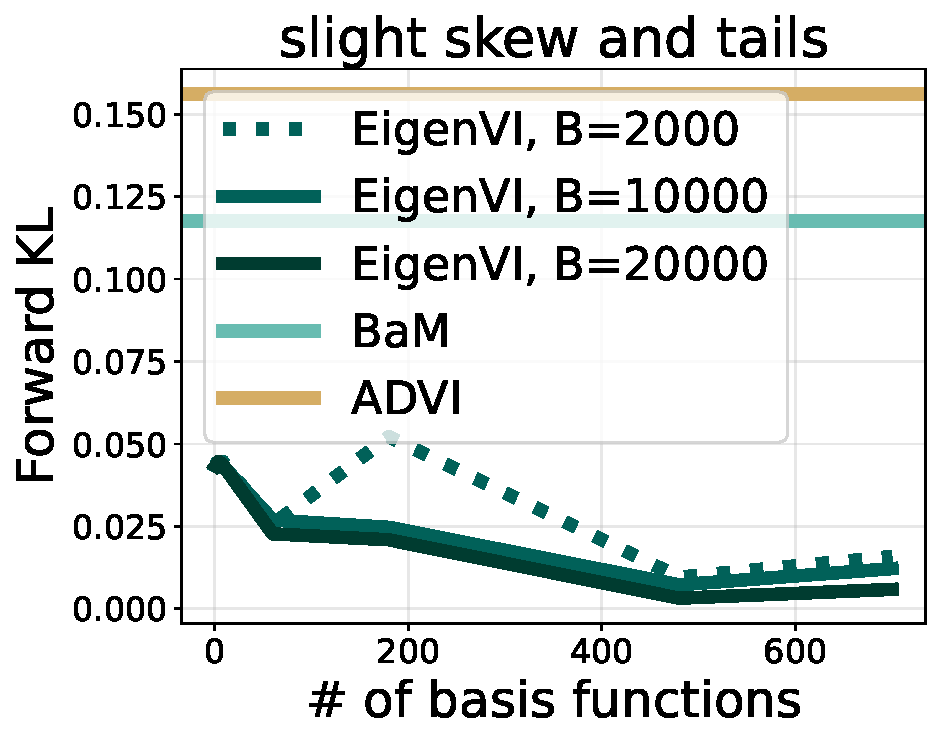
\includegraphics[scale=0.21]{figs/expts-2d/sinh-5D-P1-new.pdf}
    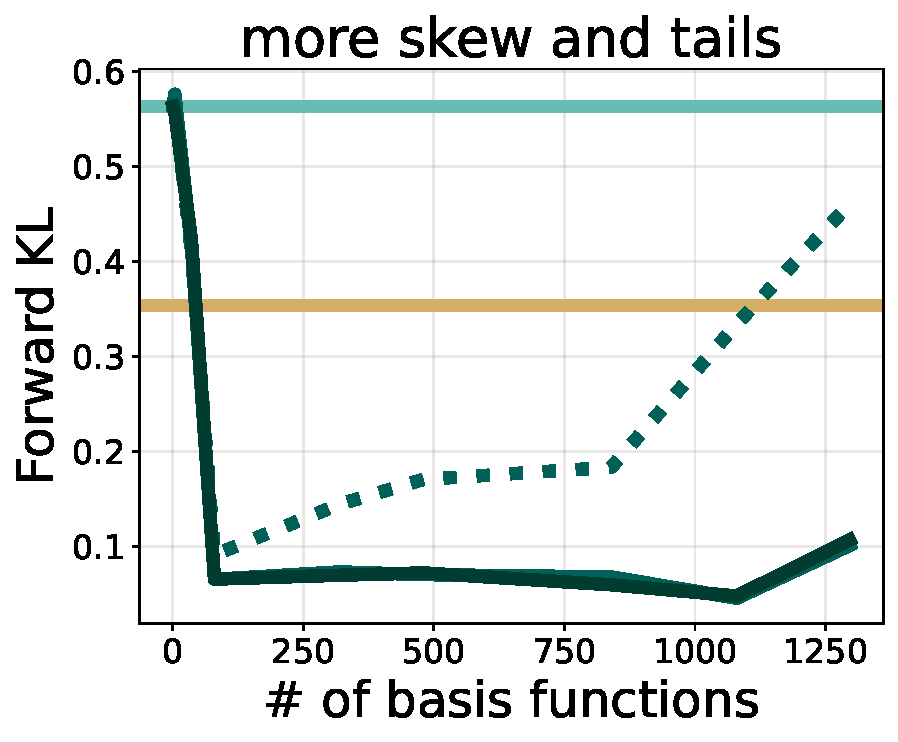
\includegraphics[scale=0.21]{figs/expts-2d/sinh-5D-P2-new.pdf}
    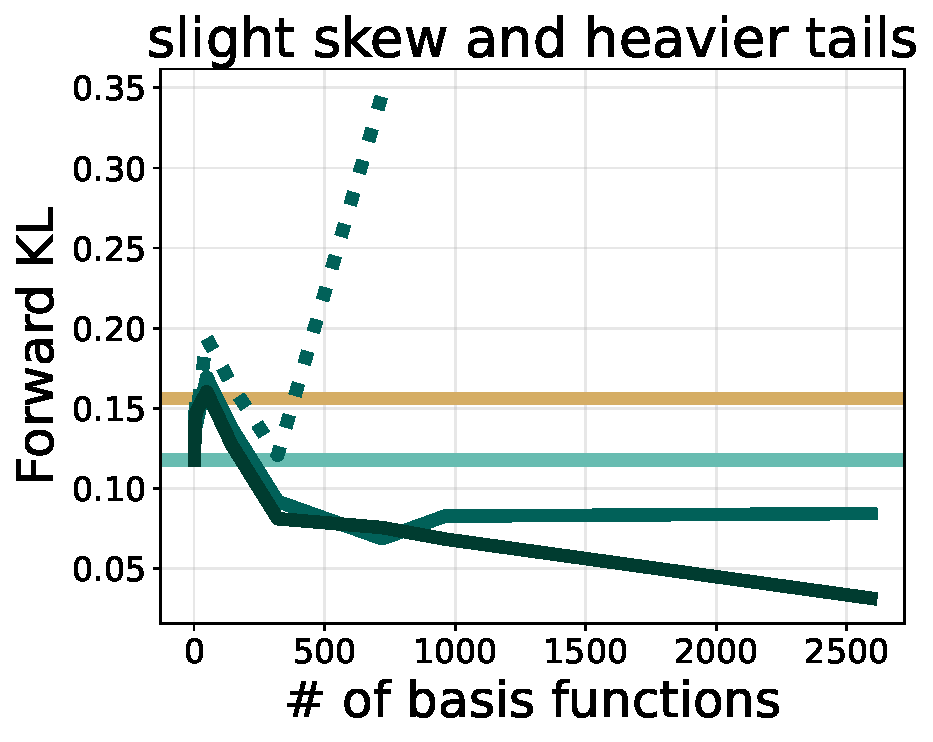
\includegraphics[scale=0.21]{figs/expts-2d/sinh-5D-P3-new.pdf}
    \caption{$D=5$}
\label{subfig:sinh5D}
    \end{subfigure}
\caption{Sinh-arcsinh normal distribution synthetic target.
    Panel (a) shows the three targets we consider in 2D, and their resulting EigenVI fit.
    Panel (b) shows measures $\KL(p;q)$ for $D=2$, and panel (c) shows $\KL(p;q)$ for $D=5$;
    the $x$-axis shows the number of basis functions, $K\!=\!\prod_d K_d$.
    }
\vspace{-12pt}
\label{fig:sinhexample}
\end{figure*}


We now consider the  sinh-arcsinh normal distribution \citep{jones2009sinh,jones2019sinh},
which is induced by transforming a multivariate Gaussian using parameters that
control the amount of skew and the weight of the tails.
%
We construct several targets ($D=2,5$) of
increasing amounts of non-Gaussianity in the skew or the tails of the distribution,
and we refer to these targets as
\emph{slight skew and tails}, \emph{more skew and tails}, and \emph{slight skew and heavier
tails}; see  \Cref{ssec-sinh} for details.
%
In \Cref{fig:sinh2dtargets},
we visualize the 2D targets and the EigenVI fits along with their forward KLs.
Before applying EigenVI, we standardize the target using a
mean and covariance estimated from batch and match VI \citep{cai2024}.
%
In \Cref{subfig:sinh2D}, we measure the EigenVI forward KL under varying numbers of samples $B$
and across increasing numbers of basis functions, given by $K\!=\!\prod_{d=1}^D K_d$.
We also present the forward KL resulting from  batch and match VI (BaM) and automatic differentiation VI (ADVI),
which both use Gaussian variational families and are run using the same budget in terms of number gradient
evaluations.
%
Next we consider similar targets with $D=5$, which are visualized in
in \Cref{fig:5dtargetdensity}, along with the resulting EigenVI variational approximations.
%
In \Cref{subfig:sinh5D},
we observe greater differences in the number of importance samples
needed to lead to good approximations, especially as the number of basis functions increase.


\subsection{Hierarchical modeling benchmarks from posteriordb}


\begin{figure*}[t]
    \centering
    \begin{subfigure}[b]{\linewidth}
        \centering
        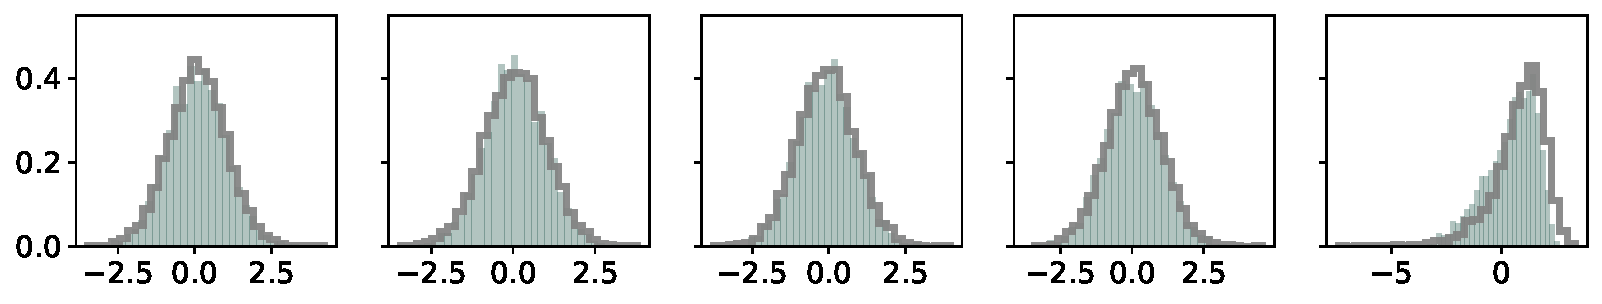
\includegraphics[scale=0.37]{figs/expts-pdb/PDB_85_samples_eigenvi.pdf}
        \caption{EigenVI with normalized Hermite polynomial family}
    \end{subfigure}
    \begin{subfigure}[b]{\linewidth}
    \centering
        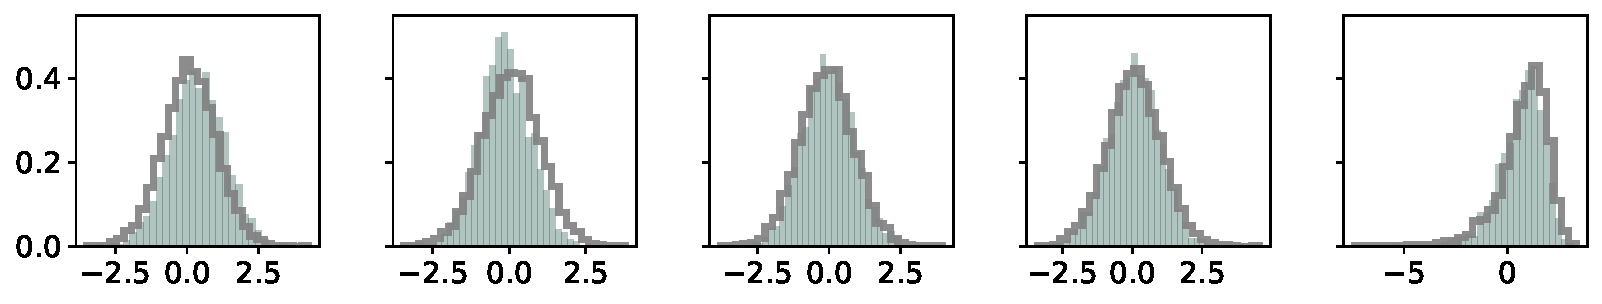
\includegraphics[scale=0.37]{figs/expts-pdb/PDB_85_samples_flows.pdf}
        \caption{VI with a normalizing flow family}
    \end{subfigure}
    \begin{subfigure}[b]{\linewidth}
    \centering
        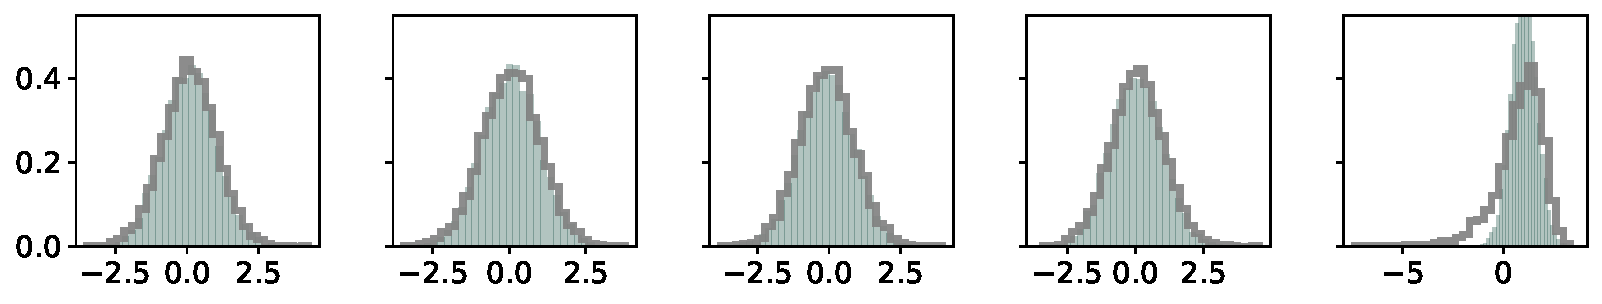
\includegraphics[scale=0.37]{figs/expts-pdb/PDB_85_samples_bam.pdf}
    \caption{Batch and match VI with a full covariance Gaussian family}
    \vspace{5pt}
    \end{subfigure}
    \begin{subfigure}[b]{0.245\linewidth}
        \centering
        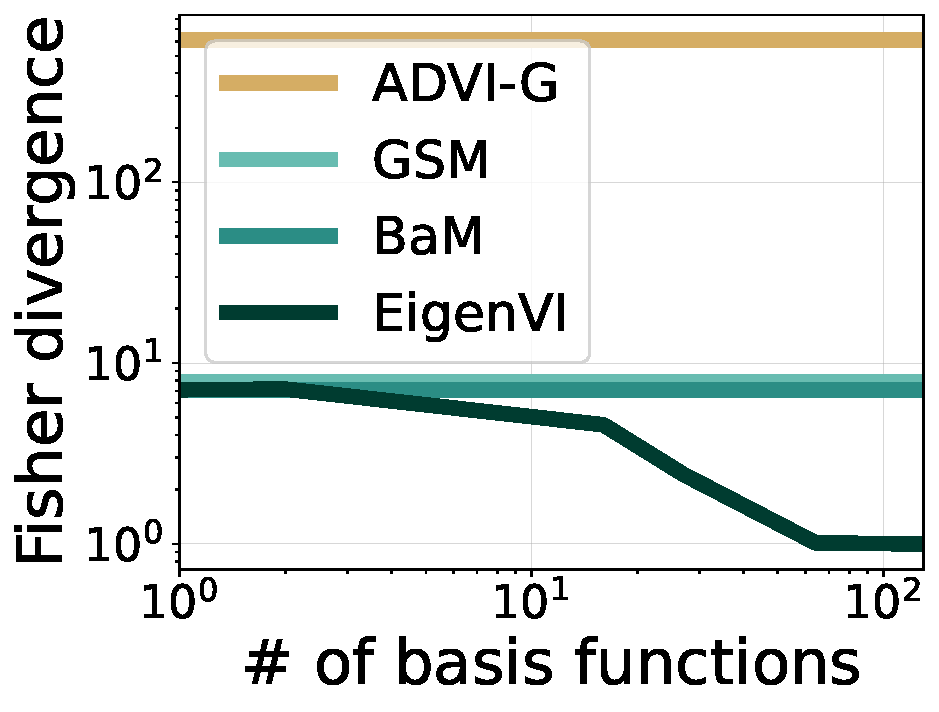
\includegraphics[scale=0.21]{figs/expts-pdb/PDB_27_scores_noflow.pdf}
    \caption{\texttt{kidscore}, $D=3$}
    \end{subfigure}
    \begin{subfigure}[b]{0.245\linewidth}
        \centering
        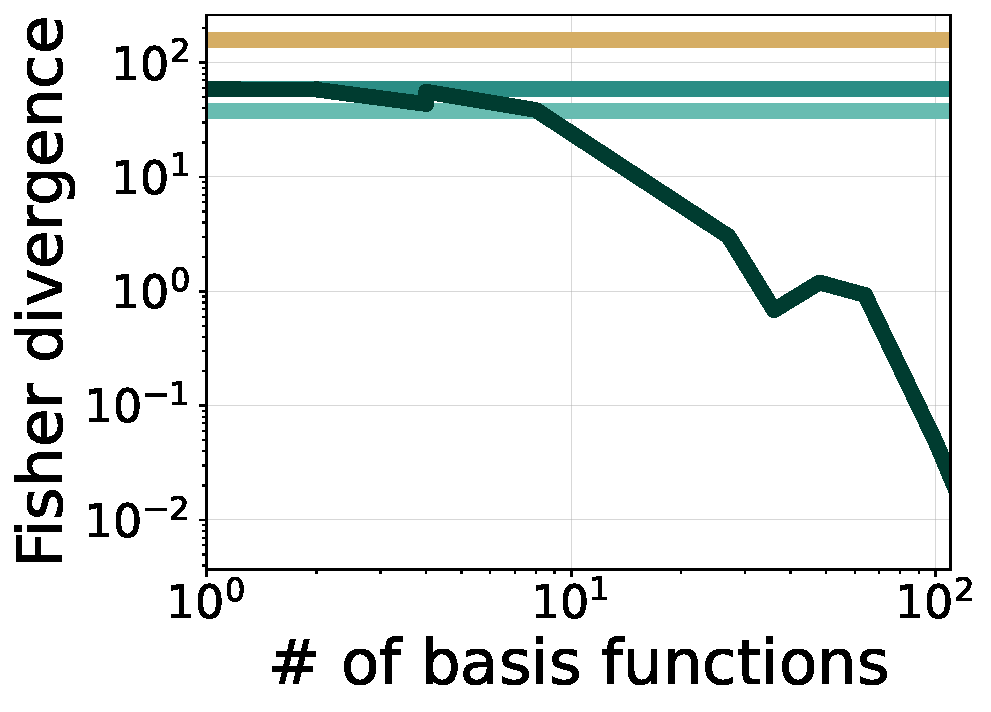
\includegraphics[scale=0.21]{figs/expts-pdb/PDB_97_scores_noflow.pdf}
    \caption{\texttt{sesame}, $D=3$}
    \end{subfigure}
    \begin{subfigure}[b]{0.245\linewidth}
        \centering
        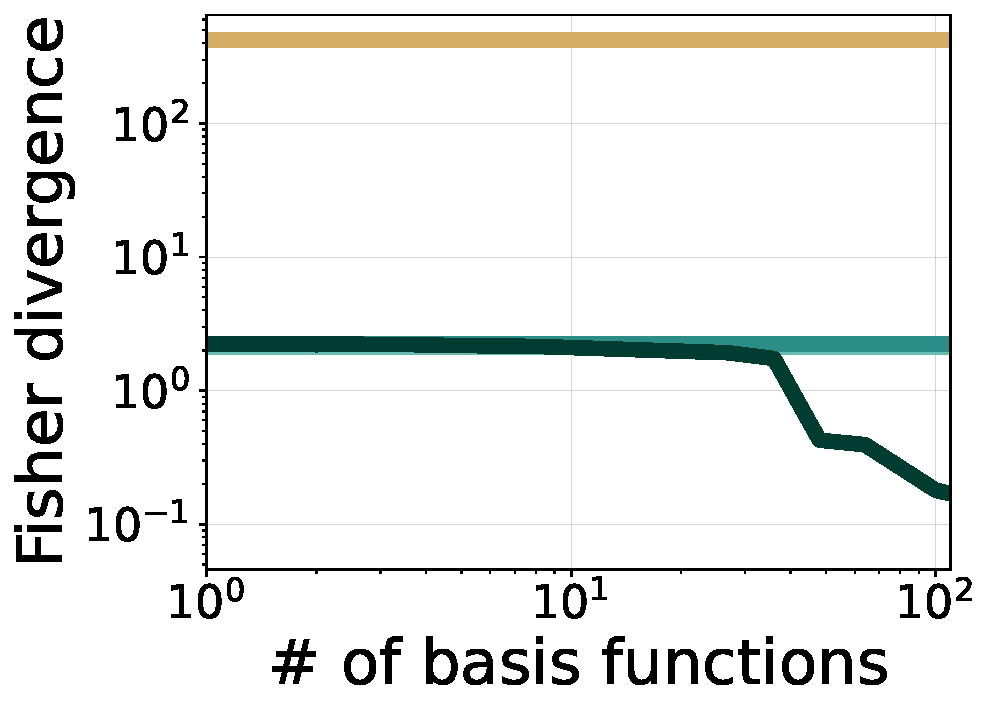
\includegraphics[scale=0.21]{figs/expts-pdb/PDB_64_scores_noflow.pdf}
        \caption{\texttt{gp-regr}, $D=3$
            }
    \end{subfigure}
    \begin{subfigure}[b]{0.245\linewidth}
        \centering
        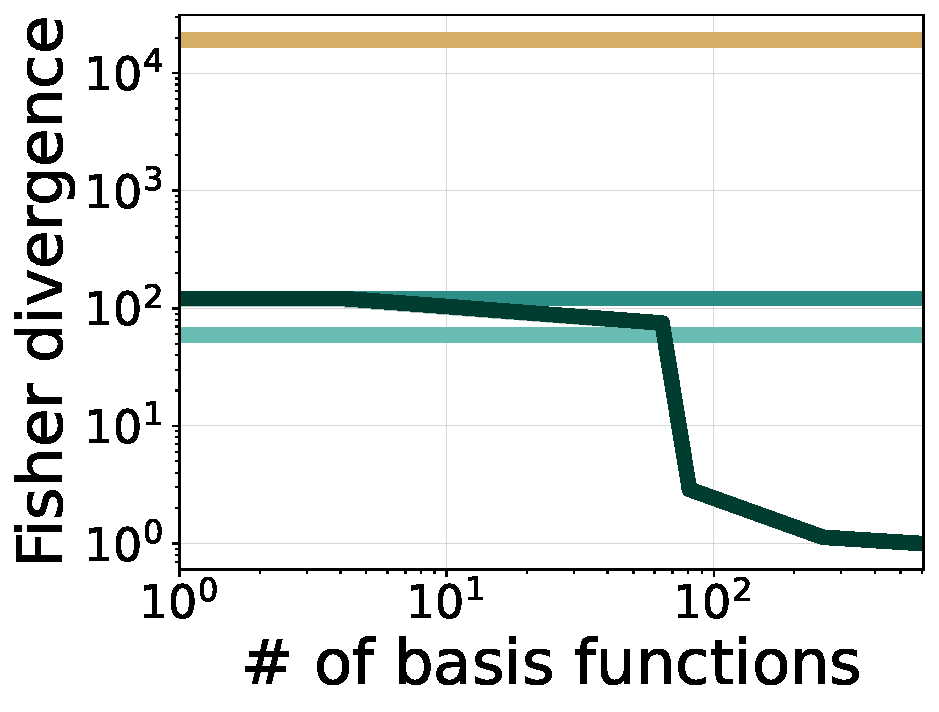
\includegraphics[scale=0.21]{figs/expts-pdb/PDB_05_scores_noflow.pdf}
    \caption{\texttt{logearn}, $D=4$}
%\caption{\texttt{earn-height}, $D=3$}
    \end{subfigure}
    \begin{subfigure}[b]{0.245\linewidth}
        \centering
        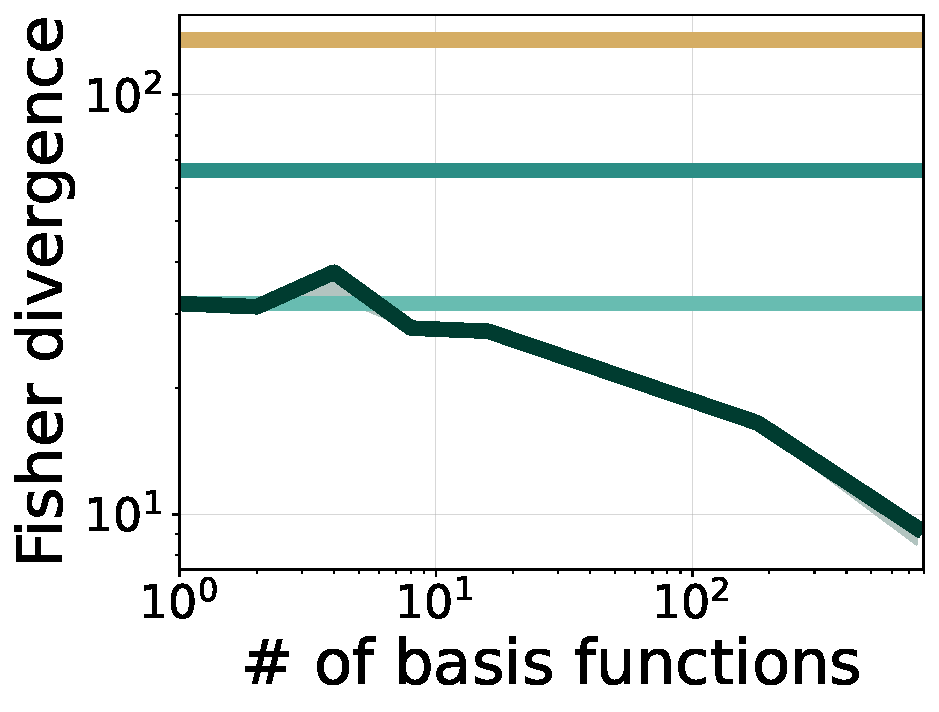
\includegraphics[scale=0.21]{figs/expts-pdb/PDB_99_scores_noflow.pdf}
        \caption{\texttt{garch11}, $D=4$}
    \end{subfigure}
    \begin{subfigure}[b]{0.245\linewidth}
        \centering
        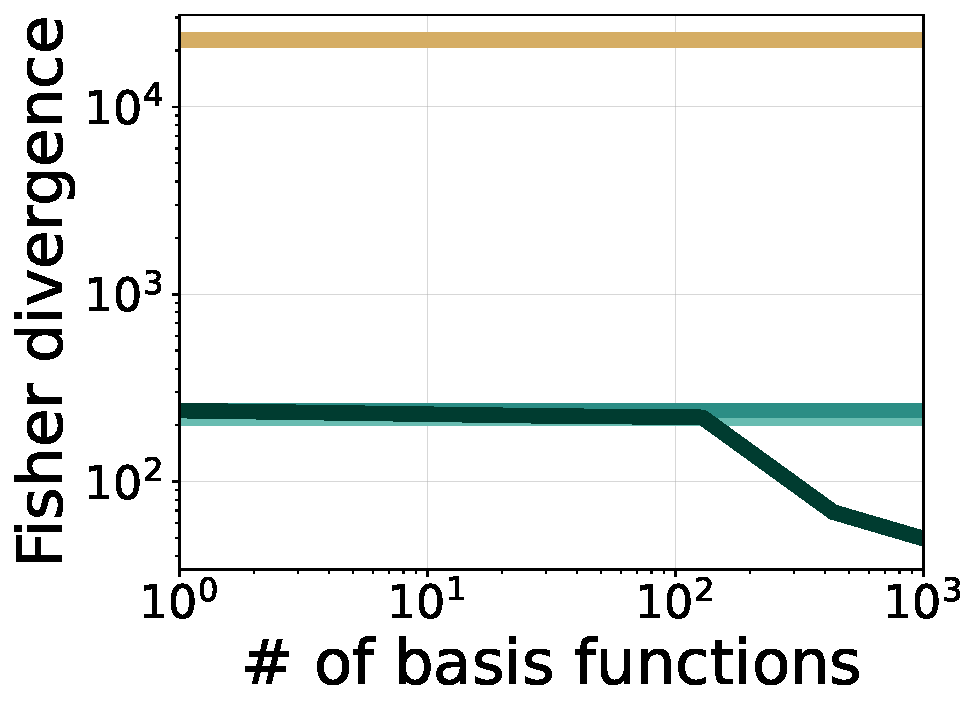
\includegraphics[scale=0.21]{figs/expts-pdb/PDB_44_scores_noflow.pdf}
\caption{\texttt{arK-arK}, $D=7$
            %(PDB-44)
            }
    \end{subfigure}
    \begin{subfigure}[b]{0.245\linewidth}
        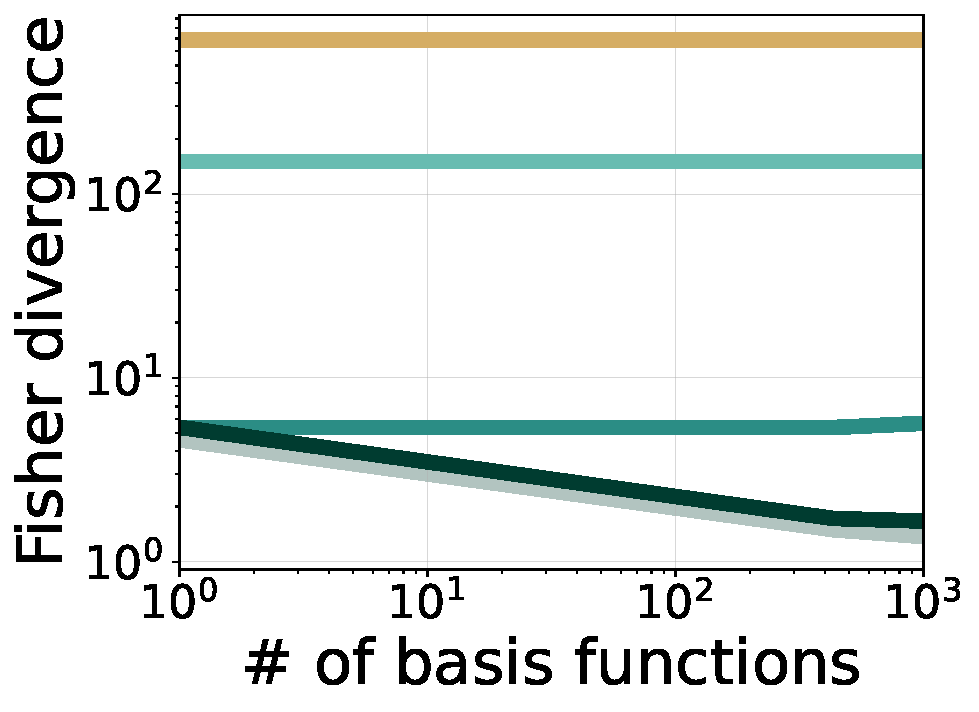
\includegraphics[scale=0.21]{figs/expts-pdb/PDB_95_scores_noflow.pdf}
    \caption{\texttt{logmesquite}, $D=7$ %(regression)
            %(PDB-95)
            }
    \end{subfigure}
    \begin{subfigure}[b]{0.245\linewidth}
        %\includegraphics[scale=0.205]{figs/expts-pdb/PDB_85_scores.pdf}
        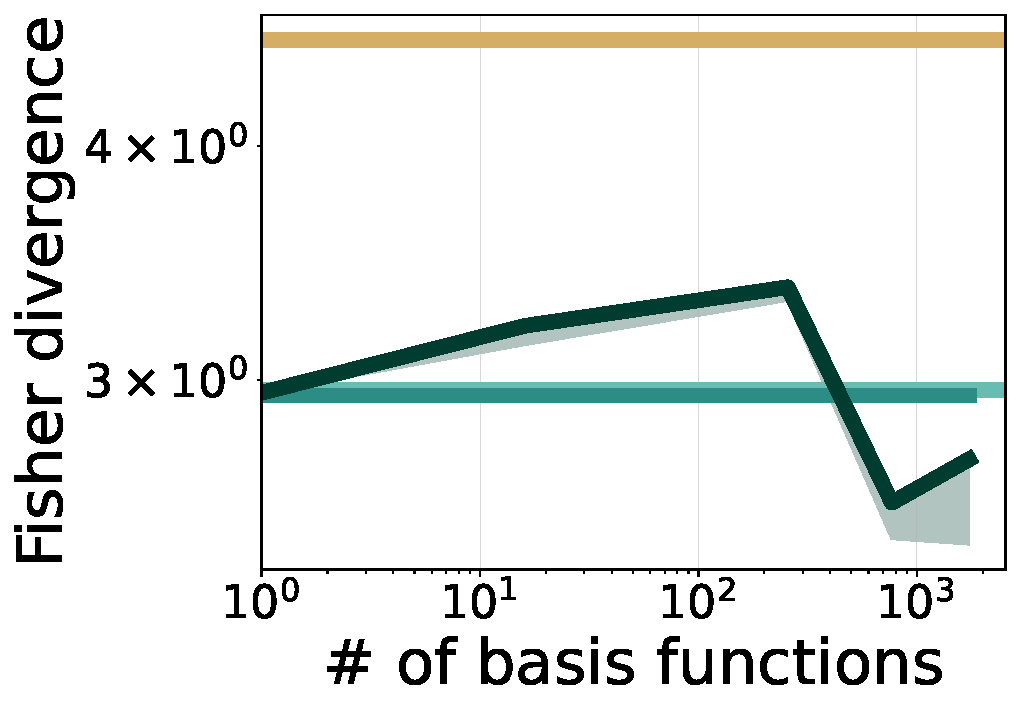
\includegraphics[scale=0.205]{figs/expts-pdb/PDB_85_scores_noflow.pdf}
    \caption{\texttt{8-schools}, $D=10$
            }
    \end{subfigure}
\caption{Results on \texttt{posteriordb} models. Top three rows:
marginal distributions of the even dimensions from \texttt{8-schools}.
Reference samples from HMC are outlined in gray, and
the VI samples are in green.
Bottom two rows: evaluation of methods with the (forward) Fisher divergence.
The $x$-axis shows the number of basis functions, $K\!=\!\prod_{d} K_d$.
Shaded regions represent standard errors computed with respect to 5 random seeds.
}
\label{fig:posteriordb}
\vspace{-10pt}
\end{figure*}

We now evaluate EigenVI on a set of hierarchical Bayesian models
\cite{carpenter2017stan,magnusson2022posteriordb,roualdes2023bridgestan},
which are summarized in \Cref{table:posteriordb}.
The goal is posterior inference: given data  observations $x_{1:N}$,
the posterior of $z$ is
\begin{align}
p(z \given x_{1:N}) \propto p(z)  p(x_{1:N}\given z) =: \rho(z),
\end{align}
where $p(z)$ is the prior and $p(x_{1:N}\given z)$ denotes the likelihood.

We compare EigenVI to
1) automatic differentation VI (ADVI) \citep{kucukelbir2017automatic}, which maximizes the ELBO over a full-covariance Gaussian family
({ADVI}),
2) Gaussian score matching ({GSM}) \citep{modi2023},
a score-based BBVI approach with a full-covariance Gaussian
    family,
and 3)
batch and match VI ({BaM}) \citep{cai2024}, which minimizes a
regularized score-based divergence over a full-covariance Gaussian
family.
In these examples, we standardize the target using either GSM or BaM
before applying EigenVI.

In these models, we do not have access to the target distribution, $p(z \given x_{1:N})$,
only the unnormalized target $\rho$.
Thus, we cannot evaluate an estimate of the forward KL.
Instead, to evaluate the fidelity of the fitted variational distributions,
we compute the empirical Fisher divergence using reference samples from the posterior
obtained via Hamiltonian Monte Carlo (HMC):
\begin{align}
\frac{1}{S} \sum_{s=1}^S \norm{\nabla \log \rho(z^s) - \nabla \log q(z^s)}^2,
    \quad z^s \sim p(z \given x_{1:N}).
\end{align}
Note that this measure is not the objective that EigenVI minimizes; it is analogous to the forward KL
divergence, as the expectation is taken with respect to $p$.
%
We report the results in \Cref{fig:posteriordb},
computing the Fisher divergence for EigenVI with increasing numbers
of basis functions.
We typically found that with more basis functions,
the scores becomes closer to that of the target.


Finally, we provide a qualitative comparison with real-NVP
normalizing flows (NFs)~\cite{dinh2016density}, a flexible variational
family that is fit by   minimizing the reverse KL.
We found that after tuning the batch-size and learning rate,
NFs generally had a suitable fit.
We visualize the posterior marginals  for a subset of dimensions from \texttt{8schools} in
the top three rows, comparing EigenVI, the NF, and BaM.
%
Here, we observe that the Gaussian struggles to fit the tails
of this target distribution.
On the other hand, EigenVI provides a competitive fit to the normalizing flow.
In \Cref{ssec:pdb},
we show the full corner plot in \Cref{fig:8schools:corner} and marginals of
the \texttt{garch11} model  in  \Cref{fig:garch11:corner}.




%\end{document}

